\documentclass{minimal}

\usepackage[latin1]{inputenc}
\usepackage{psfrag}
\usepackage{graphicx}

\begin{document}
\psfrag{X(F)}{$X(F)$}
\psfrag{F}{$F$}
\psfrag{1}{\raisebox{-1mm}{\hspace{-1mm}$\frac{1}{\tau}$}}
\psfrag{2}{\raisebox{-1mm}{$\frac{2}{\tau}$}}
\psfrag{3}{\raisebox{-1mm}{$\frac{3}{\tau}$}}
\psfrag{0}{\raisebox{-1mm}{\hspace{1mm}$0$}}
\psfrag{-1}{\raisebox{-1mm}{\hspace{-3mm}$-\frac{1}{\tau}$}}
\psfrag{-2}{\raisebox{-1mm}{\hspace{-3mm}$-\frac{2}{\tau}$}}
\psfrag{-3}{\raisebox{-1mm}{\hspace{-3mm}$-\frac{3}{\tau}$}}
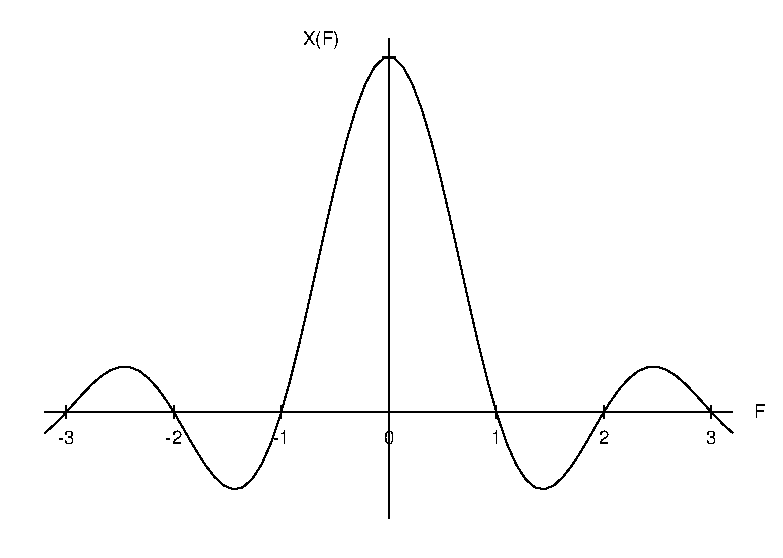
\includegraphics[scale=0.6]{prototipo_gnuplot_}
\end{document}
